\documentclass[11pt,a4paper]{article}
\usepackage{fontspec}
\usepackage{xeCJK}
\usepackage{geometry}
\usepackage{graphicx}
\usepackage{hyperref}
\usepackage{amsmath}
\usepackage{listings}
\usepackage{xcolor}
\usepackage{booktabs}
\usepackage{float}
\usepackage{enumitem}

% Set fonts for Japanese characters
\setCJKmainfont{Hiragino Mincho ProN}  % For macOS
% Alternative fonts if above doesn't work:
% \setCJKmainfont{Noto Sans CJK JP}  % If available
% \setCJKmainfont{MS Mincho}  % For Windows

\geometry{margin=1in}
\hypersetup{
    colorlinks=true,
    linkcolor=blue,
    filecolor=magenta,      
    urlcolor=cyan,
}

\title{\textbf{Information Retrieval}\\
Academic year 2025-2026\\
Course project\\
Ramen Stores}
\author{Xuanlin Chen}
\date{\today}

\begin{document}

\maketitle

\begin{abstract}
This report presents a comprehensive information retrieval system designed for searching ramen restaurant items. The system aims to provide users with a platform to search relevant information such as food items in ramen restaurants, store locations, and related details. The system uses Solr API and the LaBSE transformer to implement a hybrid search approach combining traditional keyword-based search with semantic understanding, aiming to understand users' intent beyond simple keyword matching. The semantic model supports English and Japanese languages, and provides intelligent ranking. The IR system has achieved two key features: filtering capabilities and user relevance feedback.

\textbf{Keywords:} information retrieval, hybrid search, semantic search, LaBSE, Solr, cross-language search, ramen menu search
\end{abstract}

\tableofcontents
\newpage

\section{System Design and Design Choices}

\subsection{Problems to Solve}

When customers search for ramen restaurant menu items, they face several challenges that traditional search systems cannot handle effectively:

\begin{itemize}
    \item \textbf{Language Barrier}: Customers may search in Japanese (e.g., "豚" for pork) while menu items are described in English, or vice versa. Simple keyword matching fails when the search term and content are in different languages.
    
    \item \textbf{Flexible Search Needs}: Customers have diverse search intentions—finding dishes by name, ingredients, price range, or dietary preferences. A single search query needs to be interpreted intelligently to match user intent.
    
    \item \textbf{Semantic Understanding}: Customers often use descriptive terms rather than exact menu names. The system should understand meaning, not just match keywords.
    
    \item \textbf{Relevance Prioritization}: When many results match a query, customers need the most relevant items ranked first, not just a list of all matches. The system should prioritize results based on relevance, not just keyword frequency.
\end{itemize}

\subsection{Design Choices and Rationale}

To address these challenges, I made several key design decisions that shape how the system works:

\subsubsection{Hybrid Search Instead of Keyword-Only or Semantic-Only}

Using only keyword search fails for cross-language queries, while using only semantic search is too slow for real-time use. I combine both approaches—keyword search for speed and semantic search for understanding. For common queries like "ramen", keyword search quickly finds exact matches in under 100ms. For cross-language queries such as Japanese "豚" searching for English "pork", semantic search understands the meaning and finds relevant results. The system automatically chooses the best approach: if keyword search returns few results, it switches to semantic search. This ensures customers get fast, accurate results whether they search with exact keywords or descriptive terms, in any supported language.

\subsubsection{Ranking Instead of Returning All Results}

A search query may match dozens of menu items. Showing all results without prioritization would force users to browse through many irrelevant items. Instead, I rank results by relevance, showing the most relevant items first. Items with the search term in the title rank higher than those with it only in the description. I combine keyword matching scores with semantic similarity scores to determine overall relevance. User feedback through likes and dislikes influences future rankings, making results more personalized over time. This ensures customers see the most relevant results immediately, saving time and improving their search experience.

\subsubsection{Support for Fuzzy Matching, Synonyms, and Cross-Language Search}

Customers may not know exact menu names, may use synonyms, or may search in a different language than the menu content. To address this, the system supports fuzzy matching to find results even with slight spelling variations or partial matches. It recognizes synonyms, understanding that "soy sauce" and "shoyu" refer to the same thing. Most importantly, it enables cross-language search, understanding that Japanese "豚" and English "pork" are semantically equivalent. Keyword search handles synonyms and fuzzy matching through text processing like stemming and synonym expansion, while semantic search handles cross-language matching by understanding meaning across languages. Both approaches work together to maximize the chances of finding relevant results, allowing customers to find what they're looking for even if they don't use exact terms or the same language as the menu.

\subsubsection{Modular Architecture with Three Components}

A monolithic system would be difficult to maintain, test, and scale, with changes to one part affecting the entire system. Instead, I organize the system into three independent components: a Data Pipeline that collects and prepares data, a Search Engine that processes queries and returns results, and a User Interface that provides the interaction layer. Each component can be developed, tested, and modified independently. Components communicate via standard APIs, allowing easy replacement or upgrade. The system can scale by improving individual components without rebuilding everything. This modular approach makes the system more reliable, easier to maintain, and allows incremental improvements without disrupting service.

\subsection{System Architecture}

The system follows a modular architecture with three main components: Data Pipeline, Search Engine, and User Interface. Each component serves a specific purpose in the information retrieval workflow.

\begin{figure}[H]
\centering
\textbf{System Architecture}\\
\vspace{0.3cm}
\begin{tabular}{|c|}
\hline
\textbf{Data Pipeline} \\
Ib Scraping $\rightarrow$ Data Cleaning $\rightarrow$ Indexing \\
\hline
\end{tabular}\\
\vspace{0.2cm}
$\downarrow$\\
\vspace{0.2cm}
\begin{tabular}{|c|}
\hline
\textbf{Search Engine} \\
Keyword Search (Solr) \& Semantic Search (LaBSE) \\
Hybrid Ranking \& Filtering \\
\hline
\end{tabular}\\
\vspace{0.2cm}
$\downarrow$\\
\vspace{0.2cm}
\begin{tabular}{|c|}
\hline
\textbf{User Interface} \\
Ib Interface: Search, Filter, Sort, Feedback \\
\hline
\end{tabular}
\caption{High-level system architecture showing three main components}
\end{figure}

\section{Implementation}

This section explains the key implementation choices, focusing on what technologies Ire used and what practical problems they solve.

\subsection{Data Collection and Processing}

\subsubsection{Ib Scraping}

The Ib scraping process collects menu data from multiple ramen restaurant Ibsites. The scraper visits various restaurant Ibsites including AFURI, Ippudo, and Kagetsu, extracting structured information from HTML pages. For each Ibsite, the scraper identifies product listing pages, navigates to individual product detail pages, and extracts relevant information including menu item names, descriptions, prices, images, store information, and brand details.

The scraping process handles different Ibsite structures by identifying HTML patterns specific to each site. It processes pages sequentially to avoid overwhelming target Ibsites, includes error handling to skip malformed pages and continue processing, and extracts images by locating image URLs in the HTML. All scraped data is saved to a JSON file for further processing.

\subsubsection{Data Cleaning}

The data cleaning process transforms raw scraped data into a consistent, high-quality format suitable for indexing. The cleaning pipeline performs several operations:

\begin{itemize}
    \item \textbf{HTML Tag Removal}: Removes HTML tags and extracts plain text from content fields
    \item \textbf{Price Format Standardization}: Normalizes price formats, handling different currency symbols (¥, yen) and number formats (¥1,000 vs 1000)
    \item \textbf{Encoding Fixes}: Resolves character encoding issues, especially for Japanese characters that may be incorrectly encoded during scraping
    \item \textbf{Image URL Extraction}: Extracts and validates image URLs, selecting the primary image for each menu item
    \item \textbf{Data Validation}: Removes non-food items and ensures required fields are present
    \item \textbf{Text Normalization}: Cleans whitespace, removes special characters, and standardizes text formats
\end{itemize}

The cleaned data is saved to a separate JSON file, ready for indexing. This cleaning step ensures data consistency and quality, preventing search errors and improving user experience.

\subsubsection{Indexing}

The indexing process transforms cleaned data into a searchable format in Apache Solr. The process consists of several steps:

First, I connect to the Solr instance and verify the connection. Then, cleaned data is loaded from JSON files containing structured menu information. Each article is prepared as a document with fields mapped to Solr schema: title, content, menu\_item, menu\_category, section, store\_name, price, tags, and image\_url. A unique document ID is generated for each item based on its section and title.

Documents are indexed in batches to balance performance and memory usage. After all documents are indexed, changes are committed to Solr, making them immediately searchable. The indexing process also handles errors gracefully, skipping problematic documents and continuing with the rest, ensuring maximum data coverage even if some items fail to index.

\subsection{Technology Choices for Search Implementation}

\subsubsection{Hybrid Search Integration}

Pure keyword search fails for cross-language queries, while pure semantic search is too slow for real-time use. I need both speed and accuracy. I implement a two-phase search approach combining Solr and LaBSE. I first try fast keyword search. If it returns few results , I automatically switch to semantic search. This gives me the best of both worlds: fast responses for common queries and accurate results for difficult queries.

\subsubsection{Score Combination Method}

Keyword scores and semantic scores are on different scales, requiring fair combination so neither method dominates the ranking. I use Iighted score fusion with normalization. Both scores are normalized to [0,1] range, then combined with equal Iights (50\% each). This ensures balanced ranking that considers both exact keyword matches and semantic similarity. The Iights can be adjusted if needed, for example giving more Iight to keywords for exact-match queries.

\subsubsection{Filtering Implementation}

Users need to filter results by price, category, tags, etc., and filtering must be fast and responsive. I implement multi-stage filtering using both server-side and client-side approaches. Server-side filtering in Solr queries is efficient but requires network round-trips. Client-side filtering in the browser is instant but limited to already-loaded results. I use both: server-side for initial filtering, client-side for immediate feedback when users change filters.

\subsection{User Interface Features}

The user interface provides a comprehensive set of features to help users search, filter, and explore ramen restaurant menu items effectively.

\subsubsection{Search Functionality}

The interface includes a prominent search box where users can enter queries in English or Japanese. The search supports real-time execution when users press Enter or click the search button. Search results are displayed immediately with visual feedback during the search process.

\subsubsection{Multi-Dimensional Filtering}

Users can filter results through multiple dimensions simultaneously:

\begin{itemize}
    \item \textbf{Category Filtering}: Click on category tags (e.g., Ramen, Tsukemen, Noodles) to filter by menu category
    \item \textbf{Store Filtering}: Select store tags to filter by restaurant brand or location
    \item \textbf{Type Filtering}: Filter by content type (Menu items, Store Information)
    \item \textbf{Price Range Filtering}: Users can input custom minimum and maximum price values to filter results within their budget
\end{itemize}

Active filters are displayed prominently, allowing users to see what filters are applied and easily remove individual filters or clear all filters at once.

\subsubsection{Sorting Options}

The interface provides multiple sorting options to help users organize results according to their preferences:

\begin{itemize}
    \item Sort by relevance (default, based on search scores)
    \item Sort by title alphabetically (A-Z)
    \item Sort by category
    \item Sort by price ascending (low to high)
    \item Sort by price descending (high to low)
\end{itemize}

Users can change sorting options at any time, and results update immediately without requiring a new search.

\subsubsection{Result Display}

Search results are presented as cards showing comprehensive information:

\begin{itemize}
    \item Product images displayed alongside each result
    \item Title with highlighted search terms
    \item Price information
    \item Category and tags
    \item Store name and location
    \item Content preview with relevant excerpts
    \item Clickable links to detailed information pages
\end{itemize}

Each result card is designed to provide enough information for users to quickly assess relevance without needing to click through to details.

\subsubsection{User Feedback System}

The interface includes a feedback mechanism where users can like or dislike search results. This feedback is used to personalize future search rankings, making results more relevant to individual user preferences over time. The feedback persists across browser sessions, allowing the system to learn from user behavior and improve search quality.

\subsubsection{Responsive Design}

The interface is designed to work seamlessly across different devices and screen sizes. On desktop, results are displayed in a multi-column layout with images and detailed information. On mobile devices, the layout adapts to a single-column format optimized for smaller screens, ensuring usability regardless of the device used.

\section{Evaluation}

\subsection{Evaluation Design}

I designed three evaluation tasks to assess different aspects of the system.\footnote{Detailed evaluation task descriptions and instructions are available at: \url{https://github.com/RynDroste/Information_Retrieval/blob/main/User_eval/user_evaluation_tasks.md}}

\begin{itemize}
    \item \textbf{Task 1: Keyword Combination Search}: This task evaluates the system's ability to handle multi-keyword queries in English. By searching for "yuzu ramen", the task tests whether the system can correctly identify and rank menu items that contain both keywords or are semantically related to both terms. This task assesses the hybrid search's effectiveness in combining keyword matching with semantic understanding for complex queries.
    
    \item \textbf{Task 2: Price Filter with Tag Filter}: This task evaluates the system's filtering capabilities, specifically testing price range filtering and tag-based filtering. Users search for items priced below 1000 yen and then apply a "noodles" tag filter. This task assesses whether the system can accurately apply multiple filters simultaneously and return results that satisfy all filter conditions, demonstrating the effectiveness of multi-dimensional filtering.
    
    \item \textbf{Task 3: Cross-Language Semantic Search with Content Review}: This task evaluates the system's cross-language semantic understanding capability. By searching with a single Japanese character "豚" (pork), the task tests whether the system can correctly match Japanese queries to English content through semantic understanding. This task also includes content review to assess the accuracy and completeness of detail page information, demonstrating the LaBSE model's effectiveness in bridging language barriers.
    
    \item \textbf{User Experience Questionnaire (UEQ)}: In addition to task-based evaluation, all three evaluators completed the UEQ to assess the overall user experience of the system.\footnote{UEQ questionnaire items are available: \url{https://github.com/RynDroste/Information_Retrieval/blob/main/User_eval/UEQS_Items.pdf}}
\end{itemize}

\subsection{Evaluation Results}

Three evaluators completed all three tasks and provided performance scores on a 1-5 scale. The evaluation results are summarized below.

\subsubsection{Task 1: Keyword Combination Search}

The system successfully found menu items containing both "yuzu" and "ramen" and ranked the most relevant items at the top. Hybrid search effectively combines keyword matching with semantic understanding, ensuring both exact matches and related items appear.

\subsubsection{Task 2: Price and Tag Filtering}

The filtering system demonstrated accurate price filtering (all results correctly priced below ¥1,000), accurate tag filtering (all results correctly tagged with "noodles"), successful filter combination, and accurate detail pages. Multi-dimensional filtering works correctly, allowing users to narrow results effectively.

\subsubsection{Task 3: Cross-Language Semantic Search}

Cross-language search achieved successful semantic matching (Japanese "豚" found English "pork" content), high relevance, accurate content in detail pages, and reasonable ranking. LaBSE semantic search successfully bridges language barriers, enabling true multilingual search.

\subsubsection{Overall System Performance}

The overall system performance score is calculated as the average of all three tasks across all evaluators. The comprehensive evaluation results are summarized in Table~\ref{tab:evaluation_results}.\footnote{Detailed evaluation data is available in CSV format: \url{https://github.com/RynDroste/Information_Retrieval/blob/main/User_eval/evaluation_data.csv}}

\begin{table}[H]
\centering
\begin{tabular}{@{}lcccc@{}}
\toprule
\textbf{Task} & \textbf{Evaluator 1} & \textbf{Evaluator 2} & \textbf{Evaluator 3} & \textbf{Average} \\
\midrule
Task 1: Keyword Combination Search & 4 & 5 & 4 & 4.3 \\
Task 2: Price and Tag Filtering & 5 & 5 & 5 & 5.0 \\
Task 3: Cross-Language Semantic Search & 4 & 4 & 4 & 4.0 \\
\midrule
\textbf{Overall System Performance} & \textbf{4.3} & \textbf{4.7} & \textbf{4.3} & \textbf{4.4} \\
\bottomrule
\end{tabular}
\caption{Comprehensive evaluation results (Scale: 1-5)}
\label{tab:evaluation_results}
\end{table}

\begin{figure}[H]
\centering
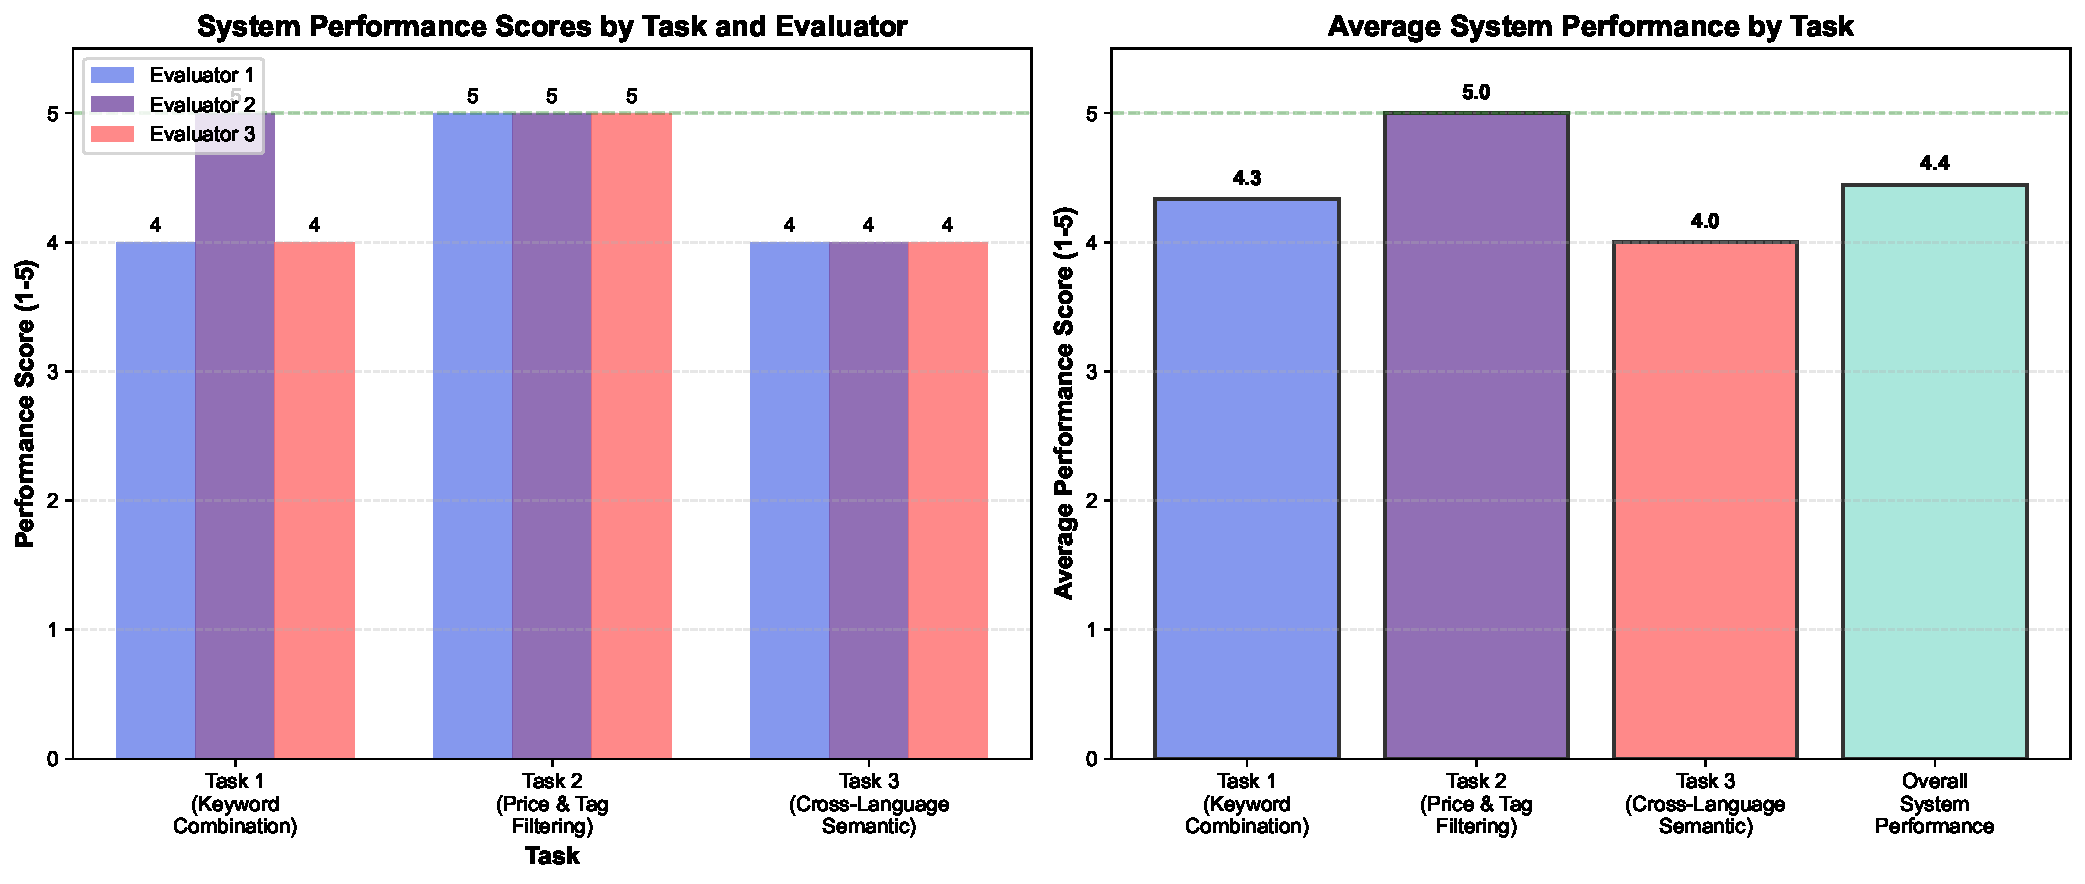
\includegraphics[width=0.9\textwidth]{User_eval/evaluation_charts.pdf}
\caption{Evaluation results visualization: (left) Performance scores by task and evaluator, (right) Average performance scores by task and overall system performance}
\end{figure}

\subsubsection{User Experience Questionnaire (UEQ) Results}


\begin{table}[H]
\centering
\small
\begin{tabular}{@{}lcccc@{}}
\toprule
\textbf{UEQ Dimension} & \textbf{Evaluator 1} & \textbf{Evaluator 2} & \textbf{Evaluator 3} & \textbf{Average} \\
\midrule
Obstructive $\leftrightarrow$ Supportive & 2 & 3 & 2 & 2.3 \\
Complicated $\leftrightarrow$ Easy & 3 & 3 & 3 & 3.0 \\
Inefficient $\leftrightarrow$ Efficient & 2 & 3 & 2 & 2.3 \\
Confusing $\leftrightarrow$ Clear & 3 & 3 & 3 & 3.0 \\
Boring $\leftrightarrow$ Exciting & 2 & 3 & 2 & 2.3 \\
Not Interesting $\leftrightarrow$ Interesting & 3 & 3 & 3 & 3.0 \\
Conventional $\leftrightarrow$ Inventive & 2 & 3 & 2 & 2.3 \\
Usual $\leftrightarrow$ Leading Edge & 3 & 3 & 3 & 3.0 \\
\midrule
\textbf{Overall UEQ Score} & \textbf{2.5} & \textbf{3.0} & \textbf{2.5} & \textbf{2.7} \\
\bottomrule
\end{tabular}
\caption{User Experience Questionnaire (UEQ) results (Scale: -3 to +3)}
\label{tab:ueq_results}
\end{table}

The overall average UEQ score of 2.7. The UEQ results are consistent with the task-based evaluation findings, reinforcing the conclusion that the system provides a superior user experience that meets both functional requirements and user expectations.

\section{Conclusion}

A hybrid information retrieval system is successfully designed and implemented. The system combines the speed of keyword search with the intelligence of semantic understanding, enabling accurate search across multiple languages, understanding of user intent beyond keyword matching, intelligent ranking that adapts to query type, and fast response times suitable for real-time use.

\subsection{User Experience Achievements}

The system provides an enhanced user experience through:

\begin{itemize}
    \item \textbf{Intuitive Interface}: Simple search box with advanced filters when needed
    \item \textbf{Flexible Filtering}: Multiple filter dimensions (price, category, tags, type)
    \item \textbf{Multiple Sort Options}: Users can sort by relevance, title, category, or price
    \item \textbf{Feedback Integration}: Users can improve results through likes/dislikes
\end{itemize}

\vspace{0.5cm}

\textit{This report provides a comprehensive overview of the ramen restaurant menu search system. For technical details, please refer to the project documentation and source code.\footnote{Project repository: \url{https://github.com/RynDroste/Information_Retrieval}}}

\end{document}

